\documentclass[10pt,a4paper]{article}
\usepackage[top=1.5cm, bottom=1.5cm, left=1.6cm, right=1.6cm, headheight=14pt, footskip=18pt]{geometry}
\usepackage[utf8]{inputenc}
\usepackage{amsmath,amsfonts,amssymb}
\usepackage{graphicx}
\usepackage{tikz}
\usepackage{circuitikz}
\usetikzlibrary{calc,patterns}
\usepackage[most]{tcolorbox}
\usepackage{enumitem}
\usepackage{fancyhdr}
\usepackage{booktabs}
\usepackage{tabularx}
\usepackage{colortbl}
\usepackage{hyperref}

% --- Palet Warna Resmi UNIB ---
\definecolor{unibblue}{RGB}{0, 32, 96}
\definecolor{unibgold}{RGB}{197, 160, 89}
\definecolor{unibgreen}{RGB}{34, 112, 60}
\definecolor{boxbg}{RGB}{248, 250, 253}
\definecolor{linegray}{RGB}{210, 215, 225}

% --- Pengaturan Header & Footer ---
\pagestyle{fancy}
\fancyhf{}
\lhead{\footnotesize\textbf{\color{unibblue}Universitas Bengkulu} \textbar\ Program Studi S1 Teknik Elektro}
\rhead{\footnotesize\color{gray}Persamaan Diferensial (Genap 2026)}
\lfoot{\footnotesize\color{gray}Lembar Kerja Mahasiswa (LKM) Berbasis OBE}
\cfoot{\footnotesize\color{gray}Hal. \thepage\ dari 2}
\rfoot{\footnotesize\color{unibblue}\textbf{Minggu 14: Fungsi Khusus}}
\renewcommand{\headrulewidth}{0.6pt}
\renewcommand{\footrulewidth}{0.4pt}

% --- Custom Box untuk Lembar Jawab ---
\newtcolorbox{answerbox}[1]{%
  colback=white,
  colframe=unibblue!70!black,
  coltitle=white,
  fonttitle=\bfseries\scriptsize,
  colbacktitle=unibblue,
  title={#1},
  arc=2pt,
  left=5pt,right=5pt,top=3pt,bottom=3pt,
  boxrule=0.6pt
}

\begin{document}

% ==================== HALAMAN 1 ====================
\noindent\begin{minipage}[c]{0.68\textwidth}%
  {\large\textbf{\color{unibblue}LEMBAR KERJA MAHASISWA (LKM)}}\\[1mm]
  {\normalsize\textbf{Mata Kuliah: Persamaan Diferensial (2 SKS)}}\\[0.5mm]
  {\small\textbf{Topik Minggu 14:} Fungsi Khusus: Persamaan Bessel \& Fenomena Efek Kulit}%
\end{minipage}%
\hfill%
\begin{minipage}[c]{0.30\textwidth}%
  \begin{tcolorbox}[colback=unibblue!5,colframe=unibblue,boxrule=0.6pt,arc=2pt,left=4pt,right=4pt,top=2pt,bottom=2pt]
    \scriptsize
    \textbf{Nama:} \dotfill\\[1.2mm]
    \textbf{NPM:} \dotfill\\[1.2mm]
    \textbf{Kelas/Klp:} \dotfill\\[1.2mm]
    \textbf{Nilai Final:} \hfill \textbf{/ 100}
  \end{tcolorbox}%
\end{minipage}\par

\vspace{1.5mm}

% Kotak Sub-CPMK & Pedoman
\begin{tcolorbox}[colback=boxbg,colframe=unibgold!90!black,boxrule=0.6pt,arc=2pt,left=5pt,right=5pt,top=3pt,bottom=3pt,title=\textbf{\scriptsize Capaian Pembelajaran (Sub-CPMK 6) \& Pedoman Evaluasi OBE}]
  \scriptsize
  \textbf{Sub-CPMK 6:} Mahasiswa mampu memecahkan Persamaan Diferensial Bessel dalam koordinat silindris serta memodelkan fenomena Efek Kulit (Skin Effect) pada konduktor ACSR sesuai IEC 61089.\\
  \textbf{Alokasi Waktu:} 50--60 Menit \quad\textbar\quad \textbf{Model:} Kolaboratif / Mandiri Terstruktur \quad\textbar\quad \textbf{Bahasa Komputasi:} Julia 1.12+
\end{tcolorbox}

\vspace{1mm}

% Soal C1
\noindent\textbf{1. (C1 - Mengingat \textbar\ Bobot: 10 Poin)}\par\vspace{0.5mm}
{\footnotesize Tuliskan bentuk baku Persamaan Diferensial Bessel berorde $n$: $x^2 y'' + x y' + (x^2 - n^2) y = 0$, dan sebutkan dua solusi bebas liniernya $J_n(x)$ (jenis pertama) dan $Y_n(x)$ (jenis kedua).}
\begin{answerbox}{Ruang Pengerjaan C1 (Bentuk Standar Persamaan Bessel \& Solusi Kanonikal)}
  \vspace{2.0cm}
\end{answerbox}

\vspace{1mm}

% Soal C2
\noindent\textbf{2. (C2 - Memahami \textbar\ Bobot: 15 Poin)}\par\vspace{0.5mm}
{\footnotesize Jelaskan mengapa fungsi Bessel jenis kedua $Y_n(x)$ harus dibuang ($C_2 = 0$) saat menyelesaikan medan fisik di dalam konduktor silinder pejal yang mencakup sumbu tengah $r=0$.}
\begin{answerbox}{Ruang Pengerjaan C2 (Prinsip Keberhinggaan Fisik Medan pada Sumbu Pusat)}
  \vspace{2.1cm}
\end{answerbox}

\vspace{1mm}

% Soal C3
\noindent\textbf{3. (C3 - Menerapkan \textbar\ Bobot: 20 Poin)}\par\vspace{0.5mm}
\noindent\begin{minipage}[t]{0.60\textwidth}%
  {\footnotesize Fenomena efek kulit pada kawat silindris berarus bolak-balik frekuensi tinggi menghasilkan persamaan rapat arus radial $J_z(r) = J_0 \frac{J_0(k r)}{J_0(k a)}$. Turunkan ekspresi kedalaman kulit (\textit{skin depth}) $\delta = \sqrt{\frac{2}{\omega \mu \sigma}}$, dan hitung $\delta$ tembaga pada frekuensi kerja $f=50\text{ Hz}$ ($\sigma = 5{,}8 \times 10^7\text{ S/m}, \mu = 4\pi \times 10^{-7}\text{ H/m}$).}%
\end{minipage}%
\hfill%
\begin{minipage}[t]{0.37\textwidth}%
  \centering
  \resizebox{0.95\linewidth}{!}{%
  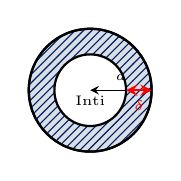
\begin{tikzpicture}[scale=0.65]
    \draw[fill=unibblue!15, thick] (0,0) circle (1.2);
    \draw[pattern=north east lines, pattern color=unibblue, thick] (0,0) circle (1.2);
    \draw[fill=white, thick] (0,0) circle (0.7);
    \draw[<->, >=stealth] (0,0) -- (1.2,0) node[midway, above, font=\tiny] {$a$};
    \draw[<->, >=stealth, red, thick] (0.7,0) -- (1.2,0) node[midway, below, font=\tiny] {$\delta$};
    \node at (0,-0.2) [font=\tiny] {Inti};
  \end{tikzpicture}%
  }%
\end{minipage}\par\vspace{1mm}
\begin{answerbox}{Ruang Pengerjaan C3 (Penurunan Kedalaman Kulit \& Perhitungan Nilai Numerik)}
  \vspace{2.8cm}
\end{answerbox}

\newpage
% ==================== HALAMAN 2 ====================

% Soal C4
\noindent\textbf{4. (C4 - Menganalisis \textbar\ Bobot: 20 Poin)}\par\vspace{0.5mm}
{\footnotesize Analisis rasio kenaikan resistansi arus bolak-balik terhadap arus searah ($R_{\text{ac}}/R_{\text{dc}}$) pada kawat transmisi daya. Jelaskan mengapa pada kabel transmisi berpenampang besar, konduktor tidak dibuat dari tembaga pejal melainkan dibuat berongga atau berpilin (*stranded*).}
\begin{answerbox}{Ruang Pengerjaan C4 (Analisis Kenaikan Resistansi AC \& Desain Geometri Konduktor)}
  \vspace{3.8cm}
\end{answerbox}

\vspace{1.5mm}

% Soal C5
\noindent\textbf{5. (C5 - Mengevaluasi \textbar\ Bobot: 20 Poin)}\par\vspace{0.5mm}
{\footnotesize Evaluasi desain konduktor ACSR (\textit{Aluminium Conductor Steel Reinforced}) menurut standar \textbf{IEC 61089}: Mengapa secara cerdas inti baja (konduktivitas rendah, kekuatan mekanik tinggi) diletakkan di bagian tengah kawat, sedangkan untaian aluminium diletakkan di lapisan luar?}
\begin{answerbox}{Ruang Pengerjaan C5 (Evaluasi Struktur ACSR Terhadap Distribusi Rapat Arus)}
  \vspace{3.8cm}
\end{answerbox}

\vspace{1.5mm}

% Soal C6
\noindent\textbf{6. (C6 - Merancang \& Komputasi Julia \textbar\ Bobot: 15 Poin)}\par\vspace{0.5mm}
{\footnotesize Rancang skrip program \textbf{Julia} menggunakan paket \texttt{SpecialFunctions.jl} untuk menghitung fungsi Bessel $J_0(x)$ dan memplot profil rapat arus radial ternormalisasi $|J_z(r)/J_0|$ dari pusat kawat ($r=0$) hingga ke permukaan kawat ($r=a$).}
\begin{answerbox}{Ruang Pengerjaan C6 (Skrip Plotting Profil Rapat Arus Radial Bessel Julia)}
  \vspace{3.8cm}
\end{answerbox}

\vspace{1.5mm}

% Tabel Rekapitulasi Skor OBE & Tanda Tangan
\noindent\begin{minipage}[b]{0.65\textwidth}%
  \centering
  \scriptsize
  \begin{tabular}{|c|c|c|c|c|c|c|}
    \hline
    \rowcolor{unibblue}
    \textbf{\color{white}C1} & \textbf{\color{white}C2} & \textbf{\color{white}C3} & \textbf{\color{white}C4} & \textbf{\color{white}C5} & \textbf{\color{white}C6} & \textbf{\color{white}Total} \\
    \rowcolor{unibblue!10}
    10 Pts & 15 Pts & 20 Pts & 20 Pts & 20 Pts & 15 Pts & 100 Pts \\
    \hline
    & & & & & & \\[2.5mm]
    \hline
  \end{tabular}%
\end{minipage}%
\hfill%
\begin{minipage}[b]{0.32\textwidth}%
  \centering
  \scriptsize
  \textbf{Verifikasi Dosen / Asisten:}\\[5mm]
  (\dotfill)
\end{minipage}\par

\end{document}
